\documentclass{beamer}
\usepackage[utf8]{inputenc}
\usepackage{fontenc}
\usepackage{graphicx}
\graphicspath{ {./"gimp imgs"} {./"screens"} }

\usetheme{POLIbeamer}


% Title Page
\title{\textsc{Fast Communication Learning Through Asymmerical Multiplayer Videogames} }
\date{21/12/2021}
\author{Jacopo Grandi}
\supervisortext{Relatore:}
\supervisor{Marco Gribaudo} 

\begin{document}

%    Title Page
\begin{frame}
\pagenumbering{gobble} 
  \titlepage
\end{frame}


\section{Introduction}
\begin{frame}
\frametitle{Serious Games}
Serious game definition:\\
	``Any piece of software that merges a non-entertaining purpose (serious) with a videogame structure (game)''
\end{frame}

\begin{frame}
\frametitle{Introduction}
Design and implemetation of a videogame that trains the communication skills of the players.
\end{frame}

\begin{frame}
\frametitle{Contents}
	\begin{itemize}
		\item Game Design
		\item Level Design
		\item Traffic Simulation
		\item Player movement: Bycicle model
		\item UDP Infrastructure
		\item State Synchronization
		\item Audio: Radio and Sounds
		\item Tests: TDD
	\end{itemize}
\end{frame}

\begin{frame}
\frametitle{Contents}
	\begin{itemize}
		\item Game Design
		\item Level Design
		\item \textbf{Traffic Simulation}
		\item Player movement: Bycicle model
		\item UDP Infrastructure
		\item State Synchronization
		\item Audio: Radio and Sounds
		\item Tests: TDD
	\end{itemize}
\end{frame}

\section{Game Design}

\begin{frame}
\frametitle{Game Design}
\end{frame}

\begin{frame}
	\begin{center}
	
		The game is set in a city with a manhattan road layout
		\\
		\medskip
		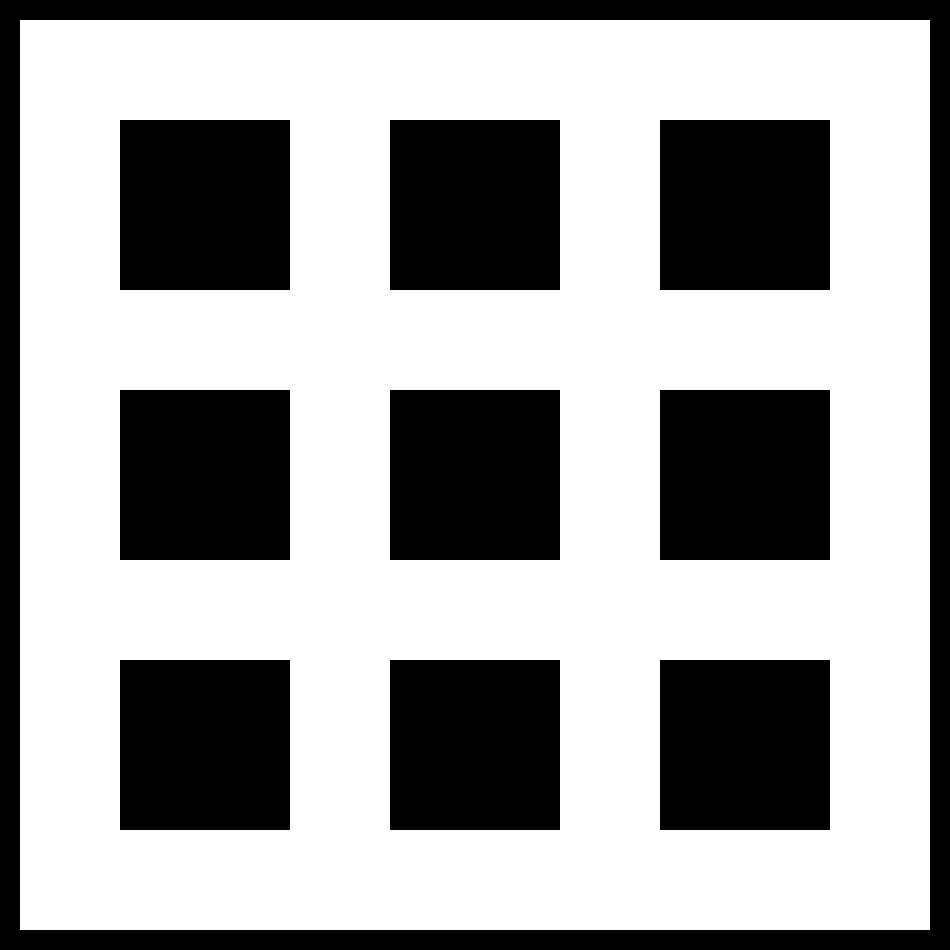
\includegraphics[height=5.0cm]{0}
	
	\end{center}
\end{frame}

\begin{frame}
	\begin{center}
	
		There are items scattered on the roads
		\\
		\medskip
		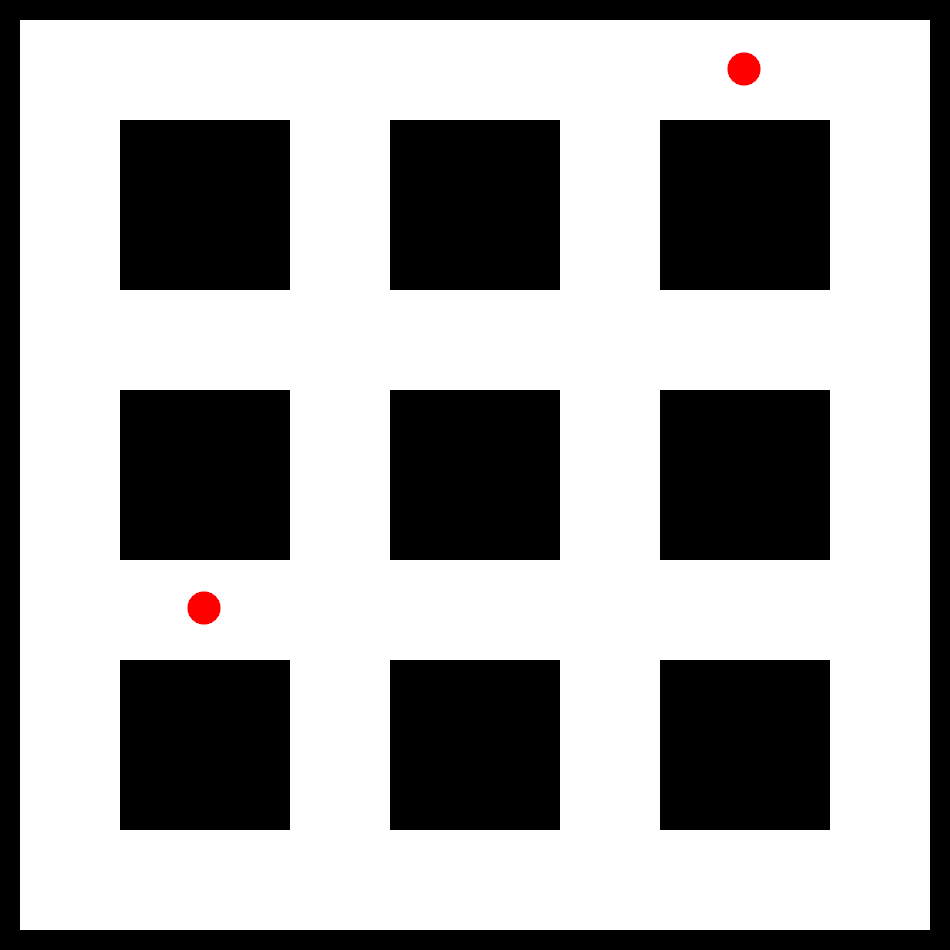
\includegraphics[height=5.0cm]{1}
	\end{center}
\end{frame}

\begin{frame}
	\begin{center}

		Items have to be carried to their destination
		\\
		\medskip
		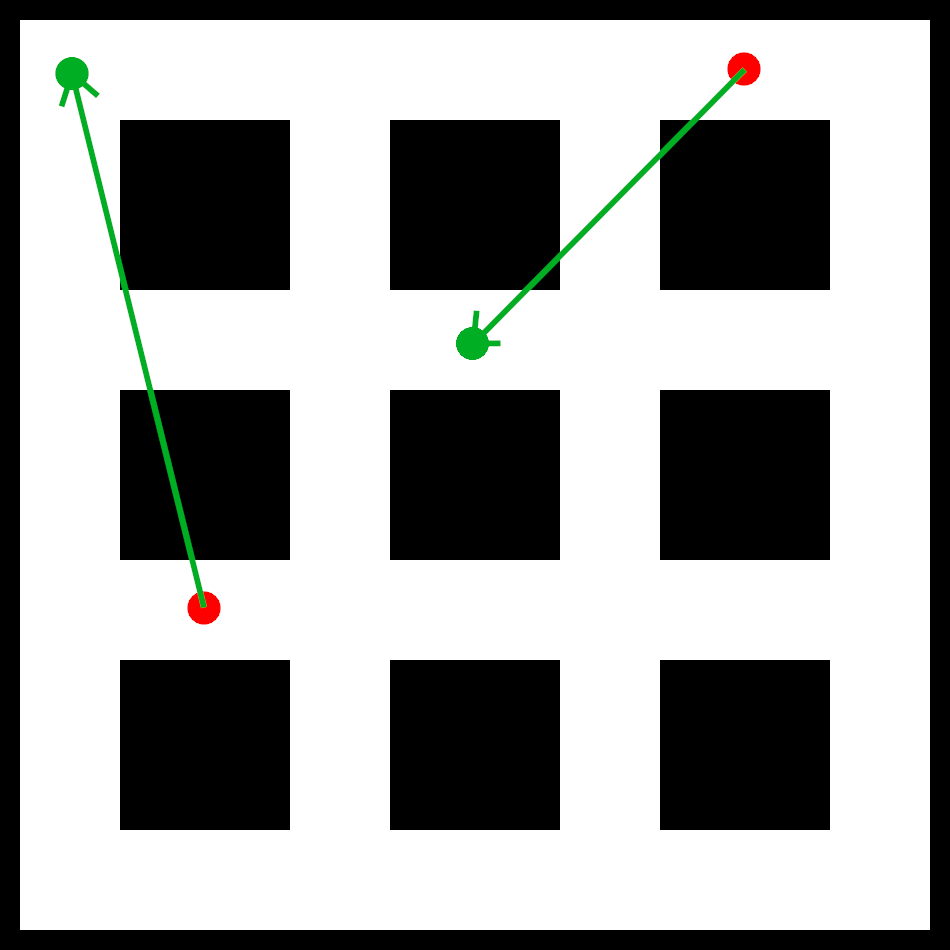
\includegraphics[height=5.0cm]{2}
	
	\end{center}
\end{frame}

\begin{frame}
The city is filled with car traffic and it's subdivided by drawbriges.
\end{frame}

\begin{frame}
The players are either Couriers or Radio Operators:
	\begin{itemize}
		\item Couriers bike through the city and carry the items
		\item Radio Operators have a map of the city
	\end{itemize}
Players can communicate by an half duplex radio.
\end{frame}

\begin{frame}
Couriers and Radio Operators have different information:
	\begin{itemize}
		\item The item location and destination is known by the Radio Operators
		\item The Radio Operators don't know the location of the Couriers
		\item The traffic levels are known to the Radio Operators
		\item The drawbridges state (open/close) is not known by the Radio Operators
	\end{itemize}
\end{frame}

\begin{frame}
The players win if they can carry all items to their destination within a time limit.
\end{frame}

\section{Level Design}

\begin{frame}
\frametitle{Level Design}
\end{frame}

\begin{frame}
	\begin{center}
	From a library of assorted 3d Models to assembled city blocks
	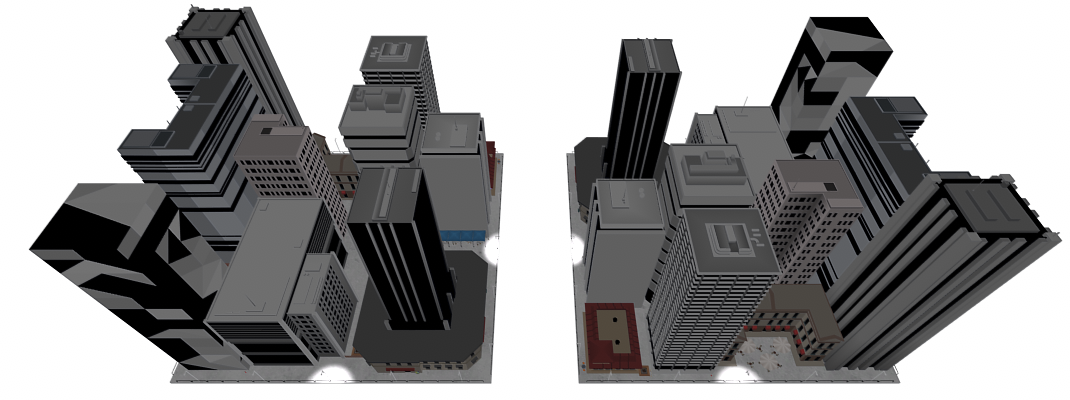
\includegraphics[width=\textwidth]{blockskyscraper}
	\end{center}
\end{frame}

\begin{frame}
	\begin{center}
	Placed to form a city
	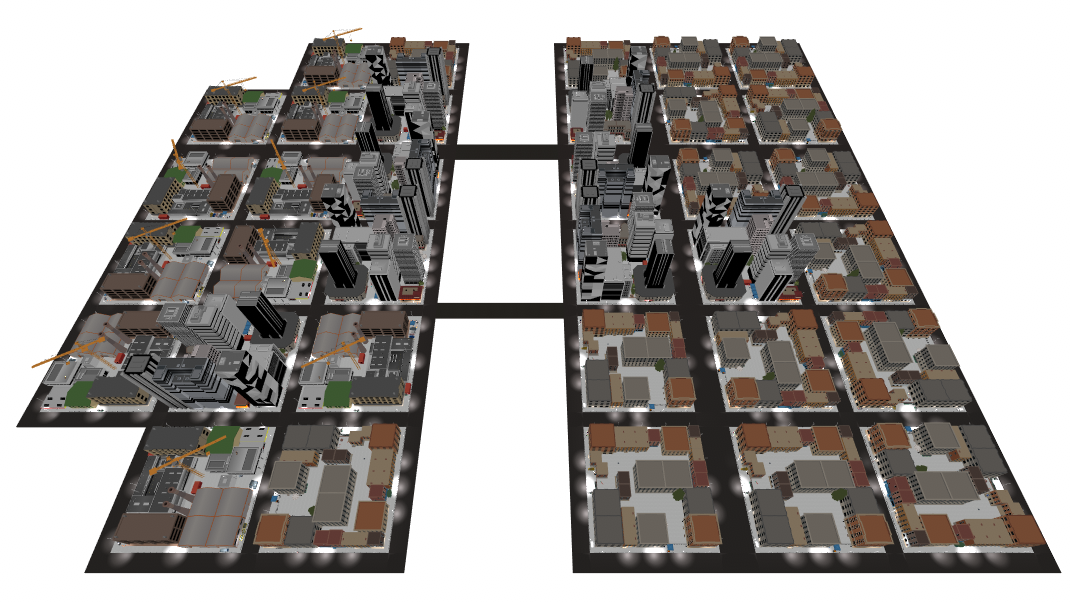
\includegraphics[width=\textwidth]{map_town}
	\end{center}
\end{frame}

\begin{frame}
	\begin{center}
	Road layout is inferred and a Road Graph is produced
	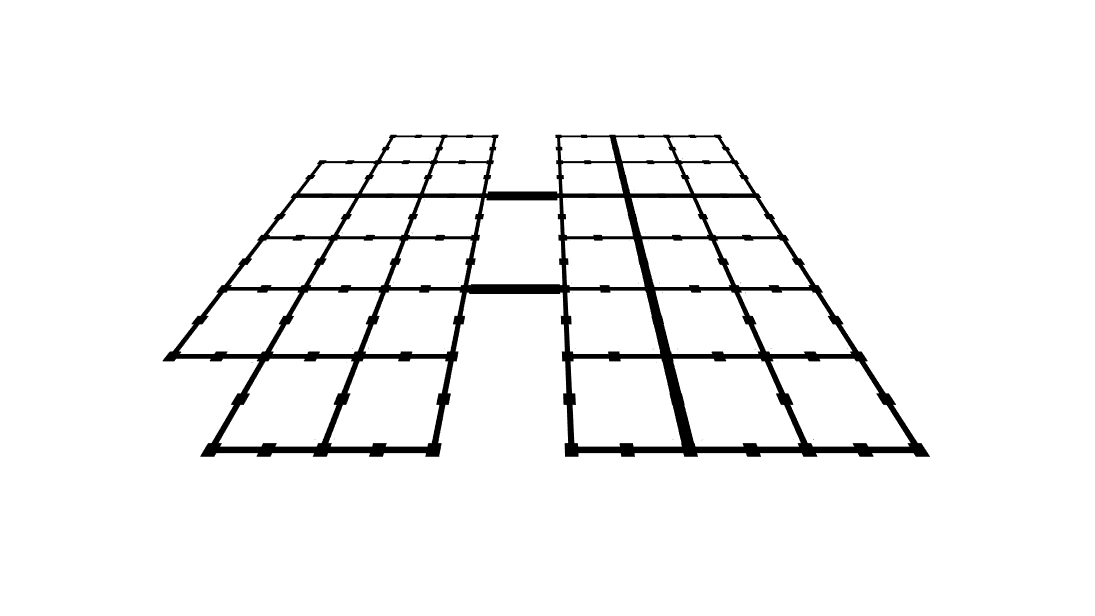
\includegraphics[width=\textwidth]{roads}
	\end{center}
\end{frame}

\begin{frame}
	\begin{center}
	Roads are named and details are placed (street signs)
	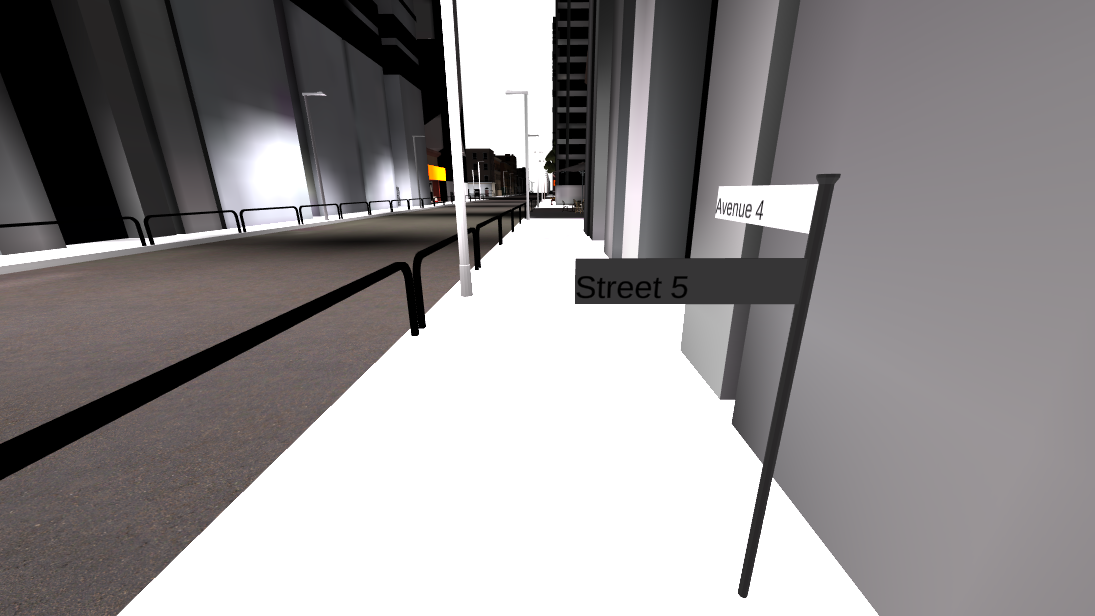
\includegraphics[width=\textwidth]{signs}
	\end{center}
\end{frame}

\section{Traffic Simulation}

\begin{frame}
\frametitle{Traffic Simulation}
\end{frame}

\begin{frame}
	\frametitle{Traffic Simulation}
	Deterministic agent based simulation. \\
	Each car is simulated as a train following the Rail Graph
\end{frame}

\begin{frame}
	\begin{center}
	Generation of the Rail Graph from the Road Graph	
	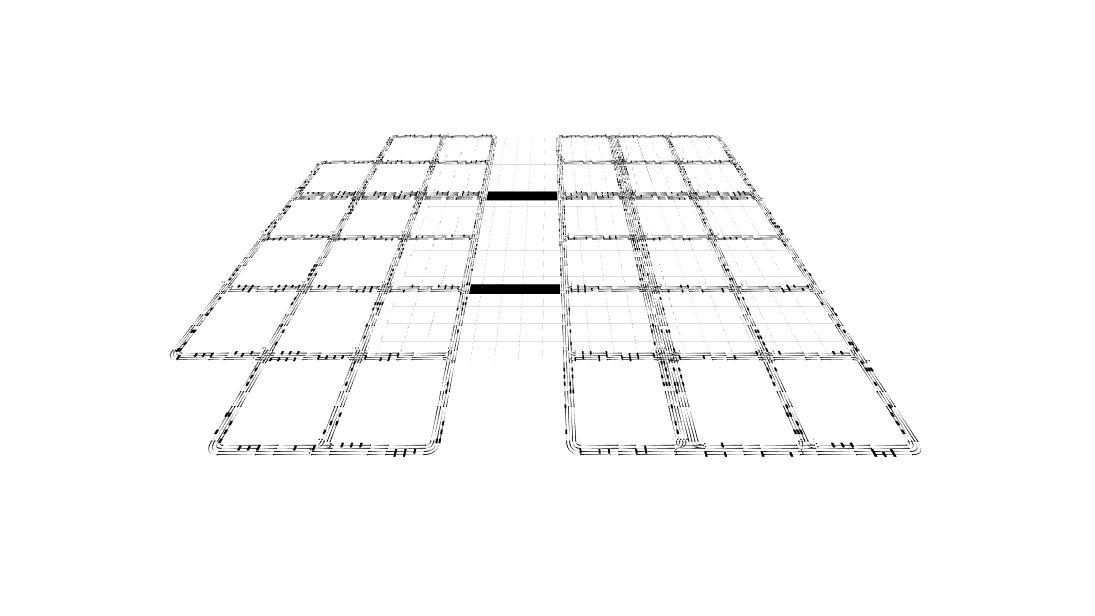
\includegraphics[width=\textwidth]{rails}
	\end{center}
\end{frame}

\begin{frame}
	\begin{center}
	4 way intersection	
	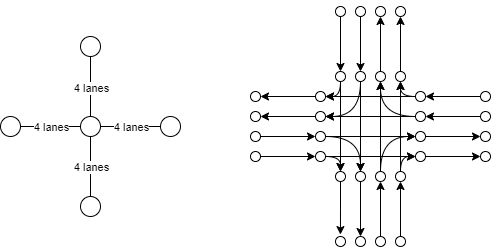
\includegraphics[width=\textwidth]{4lane}
	\end{center}
\end{frame}

\begin{frame}
	\begin{center}
	4 to 8 way intersection	
	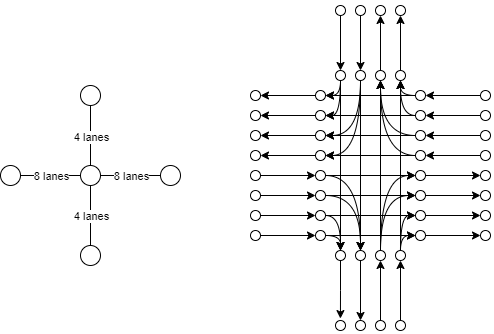
\includegraphics[width=\textwidth]{48lane}
	\end{center}
\end{frame}

\begin{frame}
	\begin{center}
	8 way intersection	
	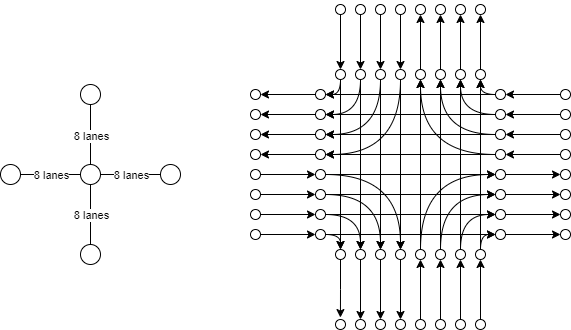
\includegraphics[width=\textwidth]{8lane}
	\end{center}
\end{frame}

\begin{frame}
	\begin{center}
	Traffic lights placement
	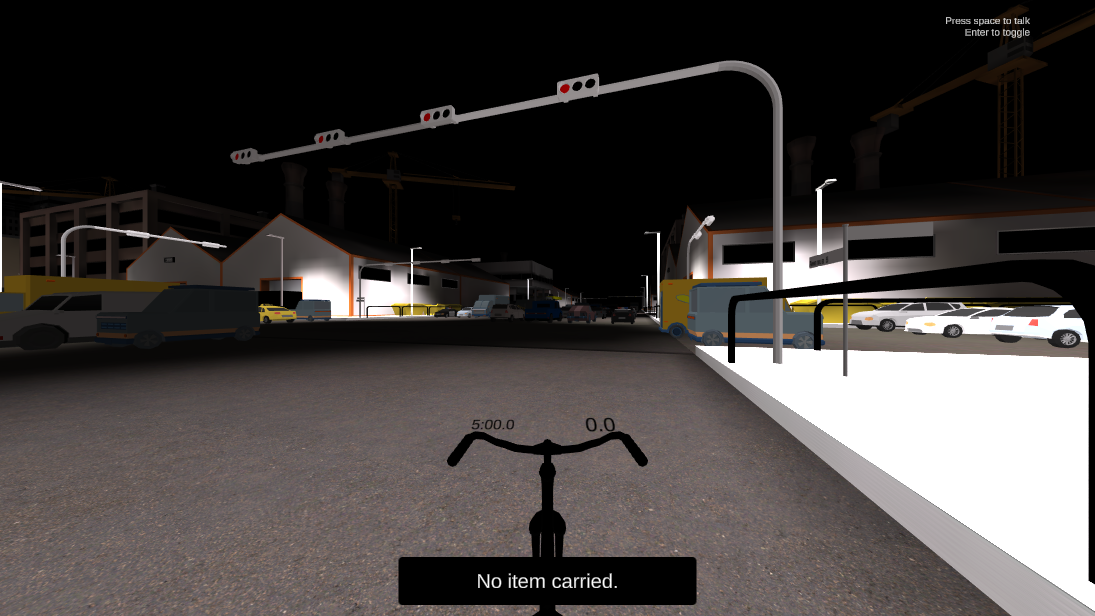
\includegraphics[width=\textwidth]{lights}
	\end{center}
\end{frame}

\begin{frame}
Car:
\begin{itemize}
	\item edge (Rail Graph)
	\item relative position
	\item velocity
	\item seed (acceleration, turn direction)
	\item absolute position calculated from edge and relative position
	\item direction (angle) calculated from edge and relative position
\end{itemize}
\end{frame}

\begin{frame}
Integration:
\begin{itemize}
	\item The simulation is integrated every 100ms
	\item It moves the cars three times and store the positions
	\item If a car is intersecting one of the other positions its not moved; otherwise, it is
\end{itemize}
\end{frame}

\begin{frame}
	Minimizing allocations and access:
	\begin{itemize}
		\item Mutable hashtables to get close to constant lookup time
		\item Indexes to lookup on graphs in constant time
		\item Precalculation of graph node stars and future car positions
	\end{itemize}
\end{frame}

\begin{frame}
	The collision detection is the simulation bottleneck. The bruteforcing approach takes \begin{math} n^2 \end{math} checks, with \begin{math} n \end{math} being the number of cars.  \\
\end{frame}


\begin{frame}
	Reducing the cars neighbors:
	\begin{itemize}
		\item Grid indexing
		\item Stopped car linking
	\end{itemize}
\end{frame}

\begin{frame}
	The collision detection and graph navigation is parallelized.
\end{frame}

\section{Bycicle Model}
\begin{frame}
	\frametitle{Kinematic Bycicle Model}
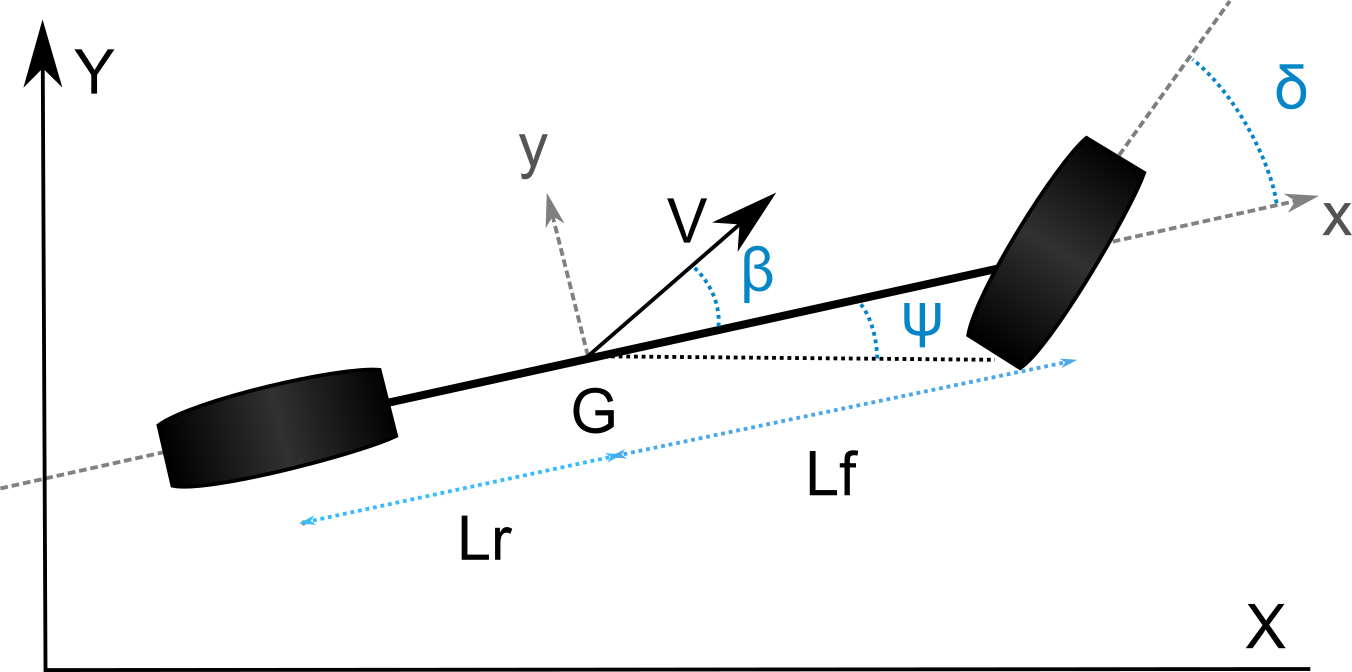
\includegraphics[width=\textwidth]{hd}
\end{frame}


\section{UDP Infrastructure}
\begin{frame}
	\frametitle{UDP Infrastructure}
UDP with reliability:
\begin{itemize}
	\item optional retransmission
	\item message fragmentation
	\item integrity check
\end{itemize}
\end{frame}


\section{Synchronization}
\begin{frame}
	\frametitle{Synchronization}
\begin{itemize}
	\item State synchronization 
	\item Stability 
	\item Interpolation (Traffic simulation)
	\item Extrapolation (Player characters)
\end{itemize}
\end{frame}

\section{Audio}
\begin{frame}
	\frametitle{Audio}
	\begin{itemize}
		\item Half duplex radio over UDP
		\item No loopback 
		\item Resampling 
		\item White noise 
		\item Hi-pass filter
		\item Traffic sound effect
		\item Bycicle sound effects 
	\end{itemize}
\end{frame}


\section{Testing}
\begin{frame}
	\frametitle{Testing}
	\begin{itemize}
\item Unit testing: TDD (Test Driven Development)
\item Integration testing: Multiplayer testing 
	\end{itemize}
\end{frame}


\end{document}
